\documentclass[11pt, a4paper]{article}
\usepackage[utf8]{inputenc}
\usepackage[margin=1.2 in]{geometry}
\usepackage{graphicx}
\usepackage[T1]{fontenc}
\usepackage{charter}
\usepackage{amsmath}
\usepackage{setspace}
\usepackage{subcaption}
\usepackage{listings}
\graphicspath{{Assets/}}

\title{CSCU9YE Assignment Report}
\author{Student no: 2519302}
\date{November 17\textsuperscript{th} 2018}
\pagenumbering{roman}
\begin{document}
\begin{titlepage}
\maketitle
\clearpage\thispagestyle{empty}
\end{titlepage}
\doublespacing
\setstretch{2}
\tableofcontents
\thispagestyle{empty}
\newpage
\singlespacing

\section{Introduction}

BIG ASS TODO

\section{Specification}

Talk through each section of the flowchart

\section{Pre-Processing}

This section will aim to cover the different aspects of pre-processing employed in this project. Within the datasets used in this project, we can see that the general steps one would need to take are as follows:
\begin{itemize}
\item Lemmatization
\item Removal of stop words
\item Removal punctuation
\end{itemize} 
Along with the aforementioned steps, the text will be processed to handle case. This is done by converting the text to lower case before any text normalization is done. 

\subsection{Lemmatization}

Lemmatization is a form of text normalization where the aim is to remove inflection and/or derive the base word from a family of words in the dataset. The base of a word, is also known as the \textbf{lemma} or the \textbf{dictionary form}. An example of which is shown in \emph{Table \ref{table: lemma}} below.\\\\
Such mapping then allows us to find all relevant documents using a specific word.
\begin{table}[h!]
\centering
\begin{tabular}{c c c}
\hline
\textbf{Word} & & \textbf{Lemma}\\
\hline
\text{Cleaning} & \(\rightarrow\) & \text{Clean}\\
\hline
\text{Cleaner}  & \(\rightarrow\) & \text{Clean}\\
\hline
\text{Cleanliness} & \(\rightarrow\) & \text{Clean}\\
\hline
\end{tabular}
\caption{Showing the mapping of words to its lemma}
\label{table: lemma}
\end{table}

\subsection{Removal of Stop Words}

Stop words are words such as "the", "he" or "in". These words do not contribute to the overall meaning of the text and are thus removed during the pre-processing stage. This also tends to be done in order to improve indexing times for larger datasets.

\subsection{Removal of Punctuation}

Punctuation, like stop words are removed due to their lack of contribution to the overall understanding of the text.  

\section{Machine Learning Methods}

This section will aim to provide some knowledge on the machine learning models employed in this project. 

\subsection{Support Vector Machine}

A Support Vector Machine (SVM) is a discriminative classification method. This method produces a classification by finding an optimal hyperplane that segregates the data points and thus returns classifications \cite{svm}. This can be visualized easiest on a 2-Dimensional plot as can be seen below in \emph{Figure \ref{fig:svm}}:
\begin{figure}[h!]
\centering
\begin{minipage}[]{0.45\textwidth}
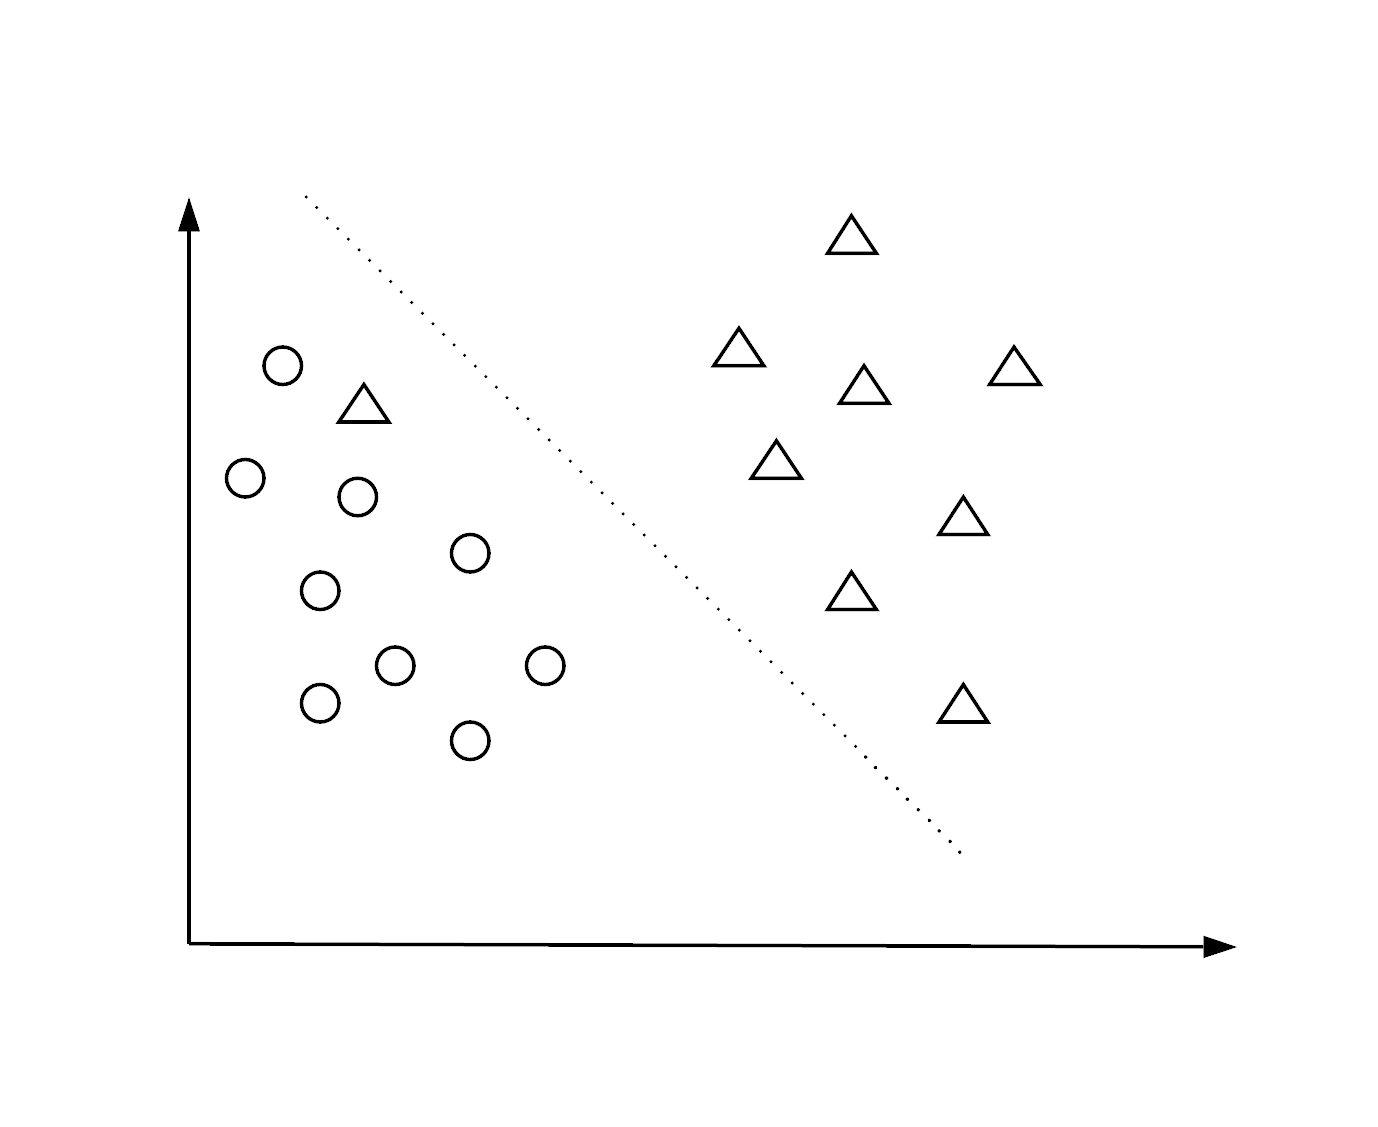
\includegraphics[scale=0.16]{svm}
\caption{SVM on 2-D plot area}
\label{fig:svm}
\end{minipage}
\hspace{0.5 cm}
\begin{minipage}[]{0.45\textwidth}
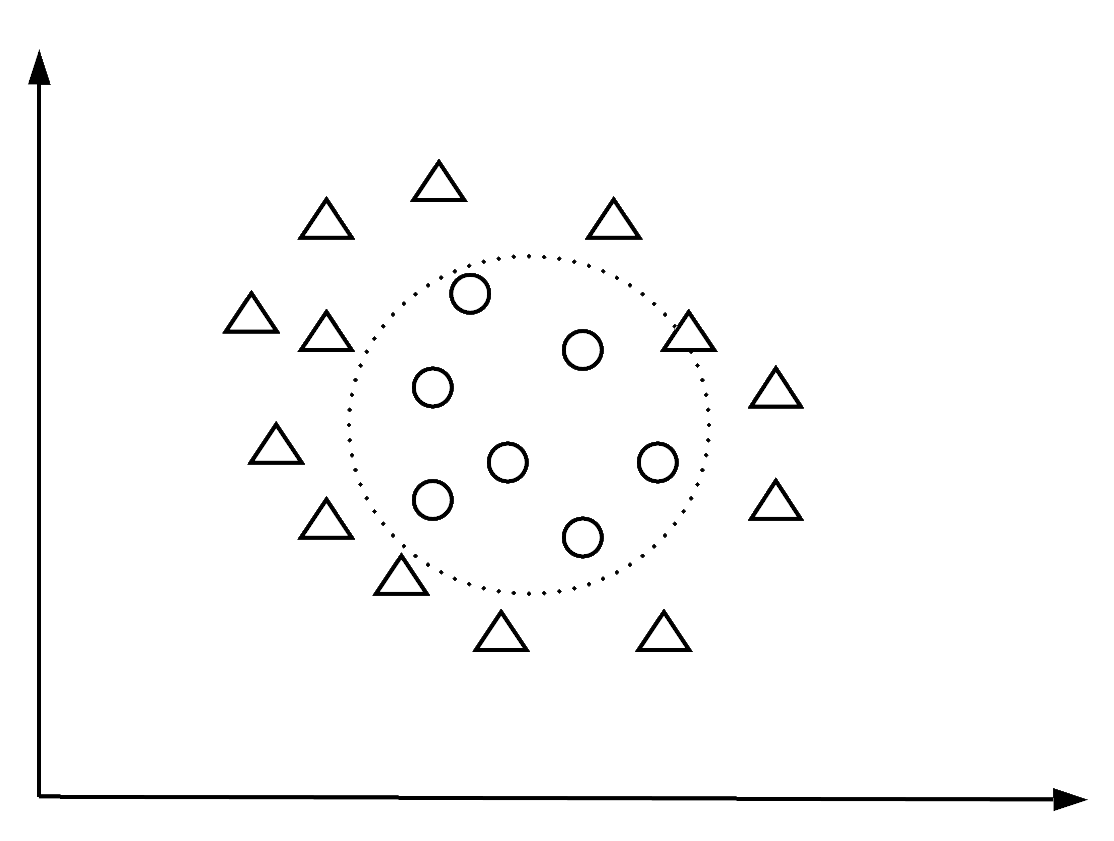
\includegraphics[scale=0.16]{svm_kernel}
\caption{Kernel feature of SVM}
\label{fig:svm_kernel}
\end{minipage}
\end{figure}

\emph{Figure \ref{fig:svm_kernel}} above shows an SVM making a classification on data where it would seem like there is no \emph{linear} hyperplane to be found. In order to make a classification, the SVM employs the kernel method \cite{ray2017svm}. This transformation, introduces a new dimension, by way of suggesting that for every \textbf{x} and \textbf{x'}, there is a function \emph{k} such that \emph{k} is equivalent to the sum of the squares of \textbf{x} and \textbf{x'} \cite{hofmann2008kernel}. This transformation then allows the model to find an optimal hyperplane within this third dimension. Transforming this back into a 2-Dimensional plot, the hyperplane is mapped as a circular boundary around the classified data points.

\subsection{Random Forest}

Random Forest is a supervised learning algorithm. The way it works is by 
  
%\section{Datasets Used} 

%\section{Measurement Metrics}

%\section{Results}
\newpage
\bibliography{references}
\bibliographystyle{ieeetr}
\end{document}
